\documentclass{article}
\usepackage{tikz}
\usetikzlibrary{calc}

\begin{document}
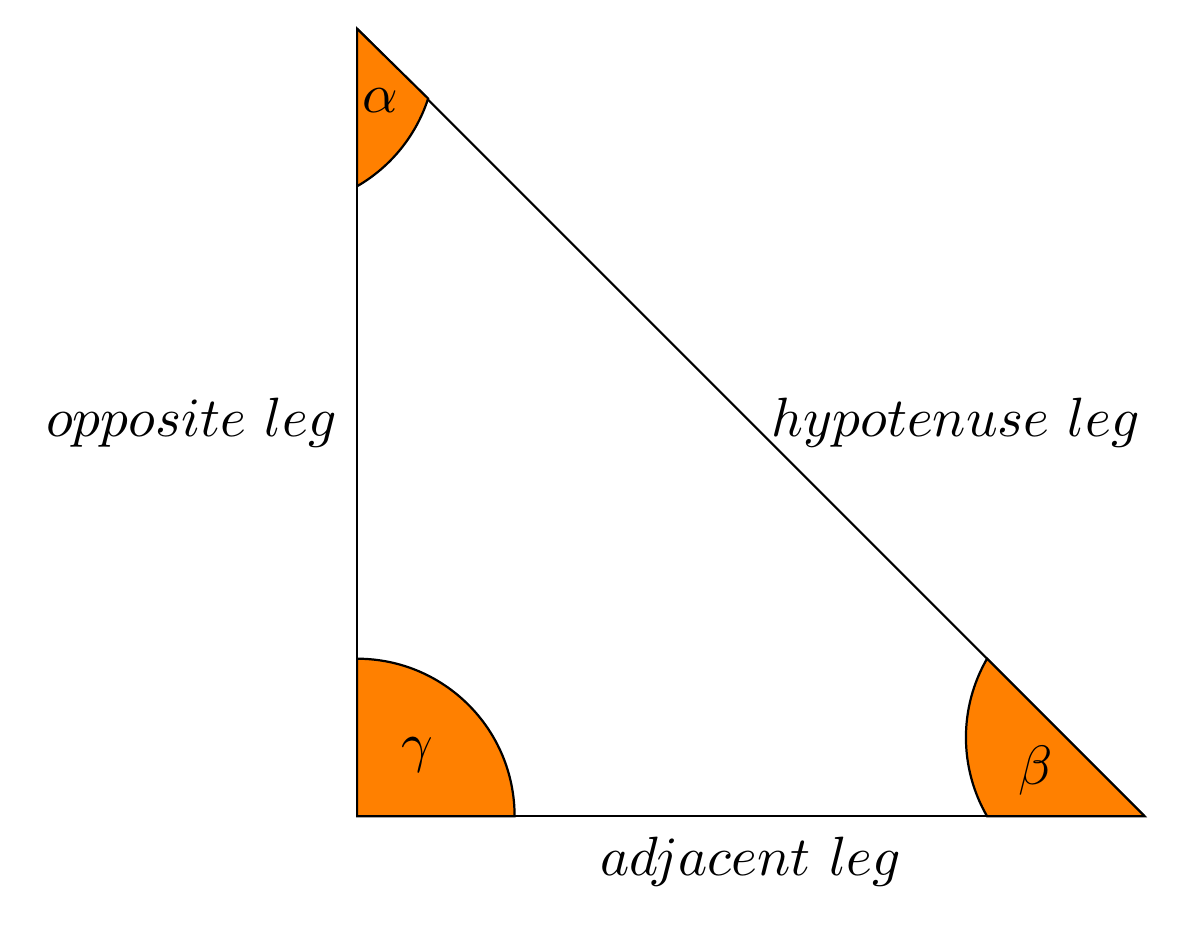
\begin{tikzpicture}[thick,scale=1, every node/.style={scale=2}]

% draw triangle
\draw(-5,-5) -- (5,-5) node[midway,below]{$adjacent\ leg$};
\draw(-5,-5) -- (-5,5) node[midway,left]{$opposite\ leg$};
\draw(5,-5) -- (-5,5) node[midway,right]{$hypotenuse\ leg$};

% angle gamma
\draw[fill=orange, thick] (-5,-5) -- (-3,-5) arc[start angle=0, end angle=90, radius=2cm] node[above right] at (-4.7,-4.7) {$\gamma$}-- cycle;

% angle alpha
\draw[fill=orange, thick] (-5,5) -- (-5,3) arc[start angle=-60, end angle=-18, radius=2cm] node[below] at (-4.7,4.5) {$\alpha$}-- cycle;

% angle beta
\draw[fill=orange, thick] (5,-5) -- (3,-5) arc[start angle=210, end angle=150, radius=2cm] node[above left] at (4.1,-5) {$\beta$}-- cycle;

\end{tikzpicture}
\end{document}
